\documentclass{article}
\usepackage[utf8]{inputenc}
\usepackage{geometry}
\usepackage{tikz}
\usetikzlibrary{positioning,arrows.meta,shapes.geometric}
\geometry{margin=0.75in}

\title{Meaning-Use Diagrams for Arithmetic Strategies}
\author{EPLE Automated Analysis}
\date{\today}

\begin{document}

\maketitle

\tableofcontents

\section{Introduction}

This document presents automatically generated Meaning-Use Diagrams (MUDs) showing how arithmetic strategies elaborate upon each other through shared computational patterns.

Each diagram shows:
\begin{itemize}
    \item \textbf{Strategy nodes} (gray rounded rectangles): Individual arithmetic strategies
    \item \textbf{Elaboration arrows}: Show how one strategy builds upon another
    \item \textbf{Pattern labels}: Computational patterns shared between strategies
\end{itemize}

\newpage

\section{Addition Strategies}

\subsection{Overview}
This diagram shows 4 addition strategies and their 6 elaboration relationships based on shared incremental counting patterns.

\subsection{Diagram}

\begin{center}
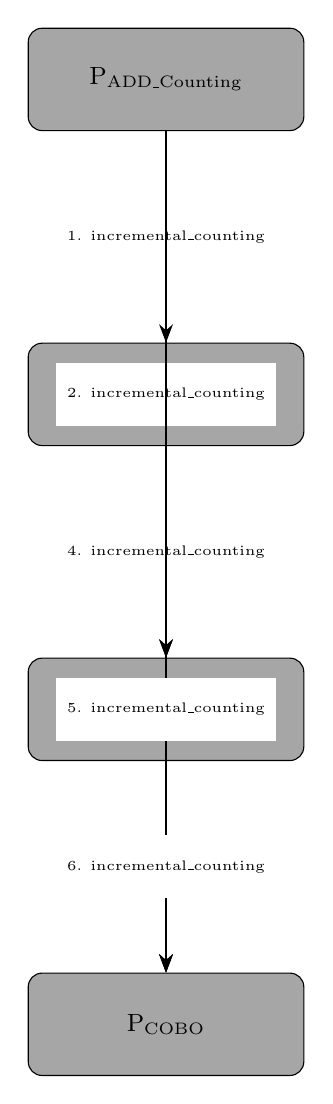
\begin{tikzpicture}[
  % Node Styles
  pnode/.style={rectangle, rounded corners=5pt, draw, fill=gray!70, text=black, minimum height=1.3cm, minimum width=3.5cm, align=center, inner xsep=0.3cm, inner ysep=0.2cm},
  graybox/.style={rectangle, fill=lightgray!50, inner sep=4pt, minimum height=0.8cm, anchor=center, align=center, text centered, font=\tiny},
  % Arrow Styles
  solidarrow/.style={-Stealth, thick},
]
\tikzset{font=\small}

% MUD Diagram for: Addition

\node[pnode] (P_ADD_Counting) at (0.00,0.00) {P\textsubscript{ADD\_Counting}};
\node[pnode] (P_ADD_Chunking) at (0.00,-4.00) {P\textsubscript{ADD\_Chunking}};
\node[pnode] (P_ADD_COBO) at (0.00,-8.00) {P\textsubscript{ADD\_COBO}};
\node[pnode] (P_COBO) at (0.00,-12.00) {P\textsubscript{COBO}};

\draw[solidarrow] (P_ADD_Counting) -- node[graybox, midway, fill=white] {1. incremental\_counting} (P_ADD_Chunking);
\draw[solidarrow] (P_ADD_Counting) -- node[graybox, midway, fill=white] {2. incremental\_counting} (P_ADD_COBO);
\draw[solidarrow] (P_ADD_Counting) -- node[graybox, midway, fill=white] {3. incremental\_counting} (P_COBO);
\draw[solidarrow] (P_ADD_Chunking) -- node[graybox, midway, fill=white] {4. incremental\_counting} (P_ADD_COBO);
\draw[solidarrow] (P_ADD_Chunking) -- node[graybox, midway, fill=white] {5. incremental\_counting} (P_COBO);
\draw[solidarrow] (P_ADD_COBO) -- node[graybox, midway, fill=white] {6. incremental\_counting} (P_COBO);

\end{tikzpicture}
\end{center}

\subsection{Interpretation}

\textbf{ADD\_Counting} serves as the foundational strategy, using basic incremental counting. This pattern is then elaborated in multiple ways:

\begin{itemize}
    \item \textbf{ADD\_Chunking}: Extends counting to work with chunks/groups
    \item \textbf{ADD\_COBO}: Counting On from Bigger Operand 
    \item \textbf{COBO}: Generic Counting On from Bigger Operand (cross-operation)
\end{itemize}

The transitive elaborations show that more complex strategies (ADD\_COBO, COBO) also share the incremental counting pattern with intermediate strategies (ADD\_Chunking).

\newpage

\section{Division Strategies}

\subsection{Overview}
This diagram shows 2 division strategies with 1 elaboration relationship based on base decomposition.

\subsection{Diagram}

\begin{center}
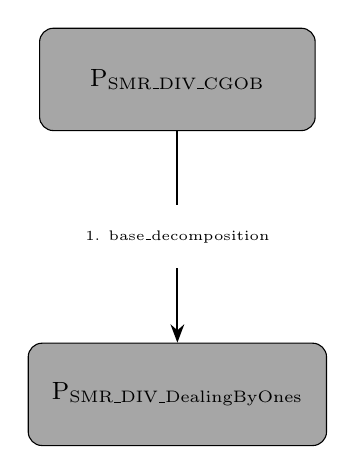
\begin{tikzpicture}[
  % Node Styles
  pnode/.style={rectangle, rounded corners=5pt, draw, fill=gray!70, text=black, minimum height=1.3cm, minimum width=3.5cm, align=center, inner xsep=0.3cm, inner ysep=0.2cm},
  graybox/.style={rectangle, fill=lightgray!50, inner sep=4pt, minimum height=0.8cm, anchor=center, align=center, text centered, font=\tiny},
  % Arrow Styles
  solidarrow/.style={-Stealth, thick},
]
\tikzset{font=\small}

% MUD Diagram for: Division

\node[pnode] (P_SMR_DIV_CGOB) at (0.00,0.00) {P\textsubscript{SMR\_DIV\_CGOB}};
\node[pnode] (P_SMR_DIV_DealingByOnes) at (0.00,-4.00) {P\textsubscript{SMR\_DIV\_DealingByOnes}};

\draw[solidarrow] (P_SMR_DIV_CGOB) -- node[graybox, midway, fill=white] {1. base\_decomposition} (P_SMR_DIV_DealingByOnes);

\end{tikzpicture}
\end{center}

\subsection{Interpretation}

\textbf{SMR\_DIV\_CGOB} (Converting to Groups of Base) uses base decomposition as its core computational pattern. This elaborates to \textbf{SMR\_DIV\_DealingByOnes}, which also employs base decomposition but in the context of distributing units one at a time.

\newpage

\section{Cross-Operation Patterns}

\subsection{Overview}
This diagram shows 2 strategies from different operations that share computational patterns.

\subsection{Diagram}

\begin{center}
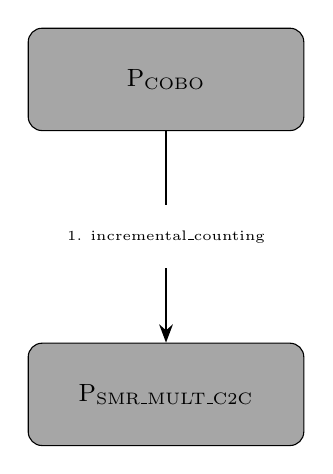
\begin{tikzpicture}[
  % Node Styles
  pnode/.style={rectangle, rounded corners=5pt, draw, fill=gray!70, text=black, minimum height=1.3cm, minimum width=3.5cm, align=center, inner xsep=0.3cm, inner ysep=0.2cm},
  graybox/.style={rectangle, fill=lightgray!50, inner sep=4pt, minimum height=0.8cm, anchor=center, align=center, text centered, font=\tiny},
  % Arrow Styles
  solidarrow/.style={-Stealth, thick},
]
\tikzset{font=\small}

% MUD Diagram for: Miscellaneous

\node[pnode] (P_COBO) at (0.00,0.00) {P\textsubscript{COBO}};
\node[pnode] (P_SMR_MULT_C2C) at (0.00,-4.00) {P\textsubscript{SMR\_MULT\_C2C}};

\draw[solidarrow] (P_COBO) -- node[graybox, midway, fill=white] {1. incremental\_counting} (P_SMR_MULT_C2C);

\end{tikzpicture}
\end{center}

\subsection{Interpretation}

This demonstrates an inter-categorial elaboration: the subtraction strategy \textbf{COBO} shares the incremental counting pattern with the multiplication strategy \textbf{SMR\_MULT\_C2C} (Count by Composites). This reveals how conceptual metaphors transcend operational boundaries.

\section{Conclusion}

These diagrams reveal the hidden structure of mathematical cognition through automated analysis of actual computational implementations. The patterns identified (incremental counting, base decomposition) serve as the pragmatic infrastructure enabling algorithmic elaboration across and within arithmetic operations.

\end{document}
